% --------------------------------------------------------------------

\section{Johdanto}

\textbf{DISCLAIMER V1:} Huonoa, muistiinpanonomaista tekstiä. Tullaan parantamaan.
\textbf{DISCLAIMER V2:} Perusasiat alkaa olla selitetty, joskin teksti on hiomatonta
ja mitä luultavimmin täynnä kirjoitus- ja lyöntivirheitä.

\newpage

\section{Aiempi tutkimus ja taustaa}



\newpage

\section{Videokoodaus}

Viimeisen viidentoista vuoden aikana suurin osa videodatasta on muuttunut
analogisesta digitaaliseksi. VHS-kaseteista ja analogisista TV-lähetyksistä
on siirrytty Blu-Ray -tekniikoihin, kännykkäkameroihin
teräväpiirtotelevisioihin. Tekniikan kehitys ei näy ainoastaan tallennusmedioissa,
sillä niin ikään tiedonsiirto on kehittynyt ja muuttunut monin paikoin
langattomaksi.(\cite{h264})
Videodatan määrä on myös valtavassa kasvussa (\cite{cisco}, \cite{youtube}).
Raaka videodata suuret määrät tallennustilaa eikä sen siirtäminen
langattomasti ole mahdollista - tarvitaan siis teknologia, jolla videodataa pakataan ja puretaan
(enkoodataan ja dekoodataan). Tätä pakkaamisen ja purkamisen prosessia
kutsutaan videokoodaukseksi. Pakkaamisen ja purkamisen lisäksi videokoodaus kattaa
myös signaalin reaaliaikaisesta kääntämisestä (transkoodaus). Transkoodaus
tarkoittaa esimerkiksi enkoodatun datan kääntämistä toiseen koodausstandardiin (\cite{mpeg_app}).
Seuraavissa alaluvuissa käsitellään videokoodausmenetelmien perusteita. Tästä lähin näihin viitataan termein
enkoodaus, dekoodaus ja transkoodaus. Toinen kirjallisuudessa esiintyvä ja
tärkeä termi on CODEC (COder DECOder pair), joka viittaa videokoodausta suorittavaan
ohjelmistoon tai laitteeseen(\cite{h264}).

Seuraavissa alaluvuissa käsitellään videokoodauksen peruskäsitteitä.

\subsection{Videokoodauksen peruskäsitteet}

\subsubsection{Videokuvan esittäminen ja tallentaminen, diskreetti kosinimuunnos}

Havaitsemamme maailma on jatkuva ja täynnä erilaisia kohteita, joilla on
erilaisia ominaisuuksia (muoto, syvyys, tekstuuri, väri, valotiheys...)
ja joita videolle haluttaisiin tallentaa. Maailma on niin niin ikään jatkuva,
mitä esimerkiksi digitaalinen maailma ei ole. Jotta kameralla tai vastaavalla
laitteella voitaisiin tallentaa esitys maailmasta, täytyy havainnot käsitellä ja
tallentaa digitaaliseen maailmaan sopivaksi. Tässä luvussa käsitellään
erialisia keinoja tallentaa videodataa - otantoja, ennustamista, väriavaruuksia
ja näihin liittyviä matemaattisia tekniikoita ja käsitteitä.

Videodataa varten maailmasta täytyy kerätä äytteitä eri ajanhetkiltä. Otanta
tapahtuu kahdessa ulottuvuudessa, ajassa ja tilassa (temporal and spatial
sampling). Tyypillisesti tilaotokset ovat suorakaiteen muotoisia kuvia
maailmasta, kun ajallinen otanta koostuu peräkkäisistä tilaotoksista.
Tilaotokset koostuvat neliönmuotoisista kuvapisteistä eli pikseleistä, jotka
on järjestetty ruudukoksi. Tilaotoksia peräkkäin toistamalla saadaan aikaan
vaikutelma elävästä kuvasta. Tällainen data (käsittelemättömät aika- ja
tilanäytteet) tunnetaan myös raakadatana. (\cite{h264})

Jokaisen tilanäytteen kuvapisteeseen tallennetaan pisteeseen liittyvät
tiedot. Yksinkertaisinta kuvaa eli mustavalkokuvaa varten riittää esimerkiksi
tallentaa vain yksi arvo kuvapisteestä (kirkkaus tai valotiheys), mutta
värikuvassa täytyy tallentaa jokaisessa pisteessä esiintyvien värien määrä.
Väriavaruudeksi kutsutaan menetelmää, joka on valittu kuvapisteiden kirkkauden,
valotiheyden ja värin kuvaamiseksi. Värikuvan tallentamisessa suosittu tapa on
RGB-väriavaruus. Tässä menetelmässä jokaisella kuvapisteellä on
kolme parametria - punaisen, vihreän ja sinisen värin määrä. Edistyneemmät
väriavaruudet hyödyntävät ihmisaivojen suurempaa herkkyyttä valotiheydelle
kuin väreille (RGB-väriavaruudessa valotiheys ja väri ovat samanarvoisia
tietoja). (\cite{h264})

Avaruudellisia näytteitä voidaan ottaa joko peräkkäin (progressive) tai
lomittain (interlacing). Peräkkäisessä otannassa jokaisella ajanhetkellä
otetaan otos, johon tallennetaan käytössä olevan standardin mukainen
määrä kuvapisteitä. Otosta kutsutaan ruuduksi (frame). Lomittaisessa
otannassa taas jokaisella ajanhetkellä tallennetaan puolet standardin
määräämistä kuvapisteistä, vaakasuunnassa joka toinen rivi siten, että
peräkkäisillä ajanhetkillä tallennetaan lomittaiset rivit. Otosta kutsutaan
kentäksi (field). Erotuksena näillä metodeilla on siinä, että lomittaisella
otannalla syntyy pehmeämmin liikkuvaa kuvaa, kuin peräkkäisellä otosten määrän
ollessa sama. Lomittamalla jokaiseen otokseen tallennetaan myös vähemmän tietoa.
(\cite{h264})

Kaikenlaiset pakkausmetodit (video, audio, kuvat) voidaan jakaa häviöttömiin
ja häviöllisiin pakkausmetodeihin (lossy, lossless). Häviöttömissä metodeissa pakatusta datasta
pystytään purkuvaiheessa palauttamaan täydellinen versio alkuperäisestä
datasta, häviöllisessä pakkauksessa purettu versio on approksimaatio
alkuperäisestä. On olemassa häviöttömiä videokoodausmenetelmiä, mutta
pakkaussuhde jää liian alhaiseksi käytännön sovelluksiin. Häviölliset
pakkausmenetelmät keskittyvät poistamaan datasta subjektiivista redundanssia,
eli sellaisia yksityiskohtia, jota havainnoija ei kykene havaitsemaan. Näin
saavutetaan huomattavasti tehokkaampia videokoodausmenetelmiä. (\cite{h264})

Suurin osa videokoodausmenetelmistä hyödyntää videodatan vahvaa
avaruudellista ja ajallista redundanssia. Käytännössä peräkkäisissä
ruuduissa on suurella todennäköisyydellä lähes samat kuvapisteet (ajallinen) ja
yhdessä ruudussa lähekkäiset kuvapisteet muistuttavat toisiaan suurella
todennäköisyydellä. Monien CODECien ensimmäinen askel videon koodaamiseen
on ennustaminen - jollakin määrällä edellisiä ajallisia näytteitä voidaan
melko suurella todennäköisyydellä ennustaa, mitä tässä näytteessä tulee
olemaan. Samaan tapaan saman näytteen sisällä jo käsiteltyjen kuvapisteiden
perusteella ennustetaan tulevien kuvapisteiden laatua. Ennustuksilla voidaan
vähentää tallennettavan datan määrää, kun purkuvaiheessa näytteitä pystytään
uudelleenrakentamaan edellisten näytteiden perusteella. (\cite{h264})

Ennen tallentamista tai siirtämistä videodataa useimmiten käsitellään vielä
jollain tavalla ennustusten lisäksi. Tavoitteena on vähentää tallentamiseen
tarvittavaa muistia ja helpottaa aikanaan tapahtuvaa dekoodausta. Tekniikoita
on monia, mutta esitellään tässä yleisin, eli diskreetti kosinimuunnos
(Discrete Cosine Transformation, DCT). 

DCT on Fourier-muunnoksen kaltainen muunnos, joka operoi $N \times N$
kokoisilla blokeilla avaruudellisissa näytteissä. Muunnos tuottaa niin
ikään $N \times N$ kokoisen blokin, mutta kuvapisteiden arvojen sijaan
uuden blokin arvot ovat kosinimuunnoksen perusblokkien suhteellisia
voimakkuuksia koodattavassa olevassa blokissa. Kuvassa \ref{fig:dct} on esitetty
$8  \times 8$ -blokin DCT:n perusblokit. (\cite{h264})

\begin{figure}[ht]
	\centering
	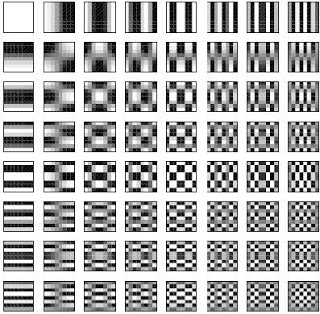
\includegraphics[width=0.5\textwidth]{dct.jpg}
	\caption{$8 \times 8$ DCT:n perusblokit}
	\label{fig:dct}
\end{figure}

DCT:n hyöty ei ole ilmeinen, sillä muunnos tapahtuu $N \times N$ -blokista
$N \times N$ -blokkiin, eikä tässä säästetä lainkaan  tilaa. Hyöty ilmenee
purkuvaiheessa - on mahdollista purkaa DCT:n avulla tallennettua tietoa
riittävän tarkaksi käyttämällä vain osaa DCT:n tuottamista suhteellisista
voimakkuuksista. Voidaan siis tallentaa vain osa DCT:n tuottamista arvoista
ja käyttää näin vähemmän tilaa tiedon tallentamiseen. Tyypillisesti käytetään
DCT:n tuottamat suurimmat arvot (merkityksellisimmät perusblokit), jolloin
harvinaisemmat ja räikeimmät erot jäävät puuttumaan lopullisesta kuvasta.
Piirtämättä jäävät sellaiset yksityiskohdat, joita ihmissilmä on muutenkin
heikko havaitsemaan. DCT:tä käyttävät koodausmenetelmät ovat siis pääosin
häviöllisiä. (\cite{h264})

DCT on Fourier-muunnoksen kaltainen muunnos, joka muuntaa videokoodauksen
tapauksessa ruutujen näyteblokkien pikseliarvoja eri taajuuksilla värähteleviksi
kosinifunktioiksi. Saavutettu etu on se, että häviöllisissä koodausmenetelmissä
voidaan jättää koodaamatta pienet korkeataajuiset funktiot - niitä ihminen
on huono huomaamaan. (\cite{h264})

\subsubsection{Videodatan matka lähteestä näyttölaitteelle, kuvadatan laadun mittarit}

Videodata saa alkunsa lähteestä, joka on tyypillisesti kamera, joka tallentaa
raakadatan. Tämän jälkeen suoritetaan CODEC suorittaa enkoodauksen, minkä
jälkeen tiivistetty data voidaan tallentaa tai siirtää. Ketjun toisessa
päässä on jälleen CODEC joka suorittaa tällä kertaa dekoodauksen ja esittää
videon käyttäjälle. Kuva \ref{fig:codec} havainnollistaa videodatan eri reittejä
käyttäjälle ja toisaalta alleviivaa sitä, että kerran koodattu data on helppo
siirtää ja se toimii erilaisissa ympäristöissä. (\cite{h264})

\begin{figure}[ht]
	\centering
	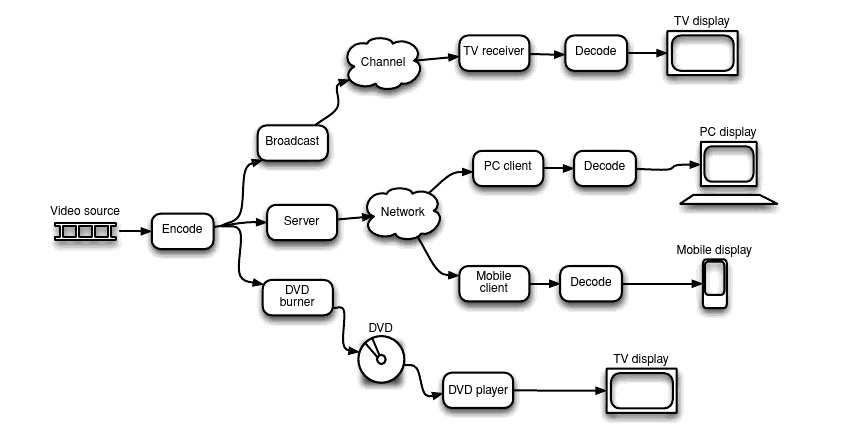
\includegraphics[width=0.5\textwidth]{codec.jpg}
	\caption{Videokoodaus mahdollistaa datan liikkuvuuden}
	\label{fig:codec}
\end{figure}

Koodauksen kolmas muoto, transkoodaus, tulisi tehdä, jos haluttu näyttölaite ei
tuekaan sille tarjottua koodaustapaa.

Videodatan laatua voidaan mitata subjektiivisesti ja objektiivisesti.
subjektiivinen mittaaminen on vaikeaa, sillä ihmisten arvioihin vaikuttavat
monet seikat. Objektiivinen mittaaminen taas antaa selviä lukuja vastaukseksi,
mutta tulosten merkitys ja vaikutus katsojakokemukseen on selvitettävä erikseen.
Videodatan kohdalla subjektiivista mittaamista voidaan usein pitää tärkeämpänä
kuin objektiivista, sillä tavoitteena usein on mahdollisimman miellyttävän
katselukokemuksen tuottaminen käyttäjälle. Toisaalta videodatan objektiivinen
laatu on erityistapauksissa myös tärkeää, esimerkiksi konenäköä hyödyntävissä
sovelluksissa. (\cite{h264})

Seuraavassa esitellään muutamia objektiivisia tapoja mitata videodatan laatua.
Subjektiivinen mittaaminen perustuu lähinnä ihmisillä tehtyihin
kyselytutkimuksiin, joilla on omat ongelmansa. Tässä työssä niihin ei keskitytä
syvemmin.

Tiheys, jolla ruutuja tallennetaan, määrää ruutunopeuden (frame rate).
Ruutunopeus ja kuvapisteiden määrä tarjoaa helpon mittarin kuvan laadulle.
Normaalitarkkuuksinen ja korkeatarkkuuksinen (Standard Definition, High
Definition) videodata eroavat toisistaan juuri kuvapisteiden määrän ja
ruutunopeuden perusteella. Valittu ruutujen tai kenttien esitystapa vaikuttaa
kuitenkin subjektiiviseen laatuun, joten ruutunopeuden ja kuvapisteiden määrää
ei voi pitää ehdottomana laadun mittarina. (\cite{h264})

Yleisesti käytetty mittari videodatan laadun mittaamiseen on PSNR-arvo (Peak
Signal to Noise Ratio). PSNR kertoo erosta alkuperäisen ja uuden kuvan välillä
ja se on määritelty

\begin{center}
$PSNR_{dB} = 10\log_{10}\frac{(2^n - 1)^2}{MSE}$,
\end{center}

missä MSE on keskimääräinen neliöity virhe (Mean Squared Error) alkuperäisen 
kuvan ja uuden kuvan välillä. (\cite{h264})

PSNR on helppo laskea ja antaa erään objektiivisen arvion videon laadusta.
Menetelmällä on puutteensa, kuten se, että alkuperäistä kuvaa ei ole
välttämättä saatavilla. Toisaalta, kuten monissa objektiivissa mittareissa,
pelkkä PSNR arvo ei vastaa suoraan mitään subjektiivista arvoa. Yleisesti
ottaen korkea PSNR arvo tarkoittaa hyvää laatua ja matala arvo huonoa.
(\cite{h264})

\newpage

\section{Rinnakkaislaskenta}

Rinnakkaislaskennan (parallel computing) tavoite on parantaa laskennan
suorituskykyä. Käsitteellisesti rinnakkaislaskentaa ei kannata sekoittaa
samanaikaiseen laskentaan (concurrent computing). Akateemisessa mielessä
jälkimmäinen keskittyy rinnakkaisen laskennan oikeellisuuteen, kun taas
ensimmäinen keskittyy saamaan hajautetusta ja rinnakkaisesta laskennasta
näkyviä hyötyjä laskentatehoon. (\cite{intro}, \cite{ari}) Tämä työ keskittyy
rinnakkaisella laskennalla saavutettuihin hyötyihin videokoodauksen saralla.

\subsection{Erilaisia rinnakkaisuuksia}

Rinnakkaisuutta on nykypäivän tietokonejärjestelmissä monella tasolla.
Nykyaikaisissa supertietokoneissa on jopa yli miljoona ydintä (\cite{top500}),
tavallisia tietokoneita kerätään laskentaklustereiksi, tieteellisessä
laskennassa hyödynnetään monenlaisia rinnakkaisia laskentamenetelmiä ja jopa
Internetiä voidaan pitää eräänlaisena rinnakkaislaskennan alustana. Toisaalta
suurten supertietokoneiden lisäksi rinnakkaisuus on tullut aivan tavallisten
kuluttajatietokoneiden osaksi. Prosessorit ovat jo pitkään hyödyntäneet
erilaisten laskentayksiköiden samanaikaista käyttöä laskentaa tehostaakseen
(pipelining, liukuhihnaus). (\cite{intro})

Yhteisiä eri tason rinnakkaisille ratkaisulle ovat niin hyödyt kuin haitatkin.
Kaikki tavoittelevat lisäystä suorituskykyyn, mutta rinnakkaisuuden
hallinta tuo laskentaan omia haasteitaan. Esimerkiksi liukuhihnaamisen hyödyt
käyvät ilmi seuraavasta esimerkistä. Oletetaan, että tehdas tuottaa autoja.
Kunkin auton valmistaminen kestää sata tuntia, joten valmistamalla yksi auto
kerrallaan saadaan sadassa tunnissa yksi auto. Jos auton valmistus kuitenkin
pilkotaan kymmeneen osaan, joita voi suorittaa rinnakkaisesti, ja joiden
suoritus kestää kymmenen tuntia, voidaankin sadassa tunnissa tuottaa kymmenen
autoa. Saavutettu hyöty triviaalissa esimerkissä on kymmenkertainen.
(\cite{intro}). Toisaalta samaa esimerkkiä voidaan hyödyntää ilmentämään
liukuhihnaamisen vaikeuksia. Jos esimerkiksi kaksi peräkkäistä tehtävää
olisivat auton ovien kiinnittäminen ja maalaaminen, niin on selvää, että autoa
ei voi maalata ennen ovien kiinnittämistä. Esimerkiksi tällaiset
riippuvuussuhteet aiheuttavat ongelmia rinnakkaislaskennalle ja niitä sekä
muita haasteita varten täytyy kehittää hallintarakenteita.

Hallintarakenteita erilaisille rinnakkaisuuden muodoille on monia.
Yksinekertaiseen liukuhihnaamiseen eräs ratkaisu on suoritettavien operaatioiden
järjestäminen sellaiseen järjestykseen, että riippuvuussuhteet eivät
aiheuta ongelmia. Toisaalta liukuhihnaa voidaan myös hidastaa, jolloin
saavutettu laskentateho vähenee, mutta laskenta pysyy oikeana. Nämä
ratkaisut kuulostavat yksinkertaisilta, mutta niiden toteutukseen ja
vaikutuksiin liittyy kuitenkin haasteita, joihin ei kuitenkaan tässä työssä
syvennytä tarkemmin. (\cite{intro})

Kun laskentayksiköitä on enemmän, tarvitaan monimutkaisempia
hallintamekanismeja. Huomattavaa on kuitenkin, että usein rinnakkaisuutta on
laskentayksikössä monella tasolla - esimerkiksi prosessoreita on monta, ja
jokaisella prosessorilla on oma liukuhihnansa. Monimutkaisemmat
hallintarakenteet voidaan jakaa karkeasti kahteen luokkaan sen perusteella,
miten paljon laskennan hallintaa kullekin laskentayksikölle on jaettu. Jos
hallinta on keskitetty, kyseessä on SIMD-arkkitehtuuri (Single Instruction
stream, Multiple Data stream). SIMD-arkkitehtuurissa yksittäinen
hallintayksikkö päättää, mitä kukin laskentayksikkö laskee.
MIMD-arkkitehtuurissa (Multiple Instrucrion stream, Multiple Data stream)
jokaisella laskentayksiköllä on oma hallintayksikkönsä. Konkreettisena
esimerkkinä arkkitehtuurien erona voi pitää esimerkiksi sitä, että
MIMD-arkkitehtuurissa jokainen laskentayksikkö voi suorittaa eri ohjelmia, kun
SIMD-arkkitehtuurissa hallintayksikkö päättää, mitä ohjelmaa kaikki
laskentayksiköt suorittavat. (\cite{intro})

\subsection{Rinnakkaisuuden peruskäsitteitä}

Erilaisten rinnakkaisuuden muotojen lisäksi rinnakkaislaskenta voidaan jakaa
kahteen tyyppiin sen perusteella, mihin rinnakkaisuus kohdistuu.
Tehtävärinnakkaisessa laskennassa rinnakkain suoritetaan erilaisia
tehtäviä - esimerkiksi saman ohjelman eri säikeitä. Datarinnakkaisessa
ohjelmoinnissa taas rinnakkaisuus syntyy siitä, että operoidaan samaan aikaan
eri datan osa-alueilla. \cite{intro} Datarinnakkainen lähestymistapa sopii varsin hyvin
videokoodauksen rinnakkaistamiseen - jos esimerkiksi tehdään DCT, voidaan
kukin blokki käsitellä erikseen (blokit ovat riippumattomia toisistaan), joten
saavutetut hyödyt laskenta-ajassa ovat huomattavat.

Rinnakkaisuuden kohteen lisäksi rinnakkaisilla kohteilla on erilaisia tapoja
järjestää tiedon liikkuminen laskentayksiköiden välillä. Pääparadigmoja on
kaksi, jaettu muisti ja viestinvälitys. Jaetun muistin mallissa
laskentayksiköillä on yhteinen muisti, josta jokainen saa lukea ja kirjoittaa.
Jotta yhteinen muisti pysyy puhtaana (kaksi laskentayksikköä ei lue ja/tai
kirjoita samaan muistiosoitteeseen samaan aikaan), täytyy järjestelmällä
olla keinot päättää, milloin mitäkin muistialuetta saa käsitellä.
Erilaisia ratkaisuja tähän ongelmaan (mutual exclusion) on useita, kuten
monitorit tai semaforit. Samojen muistialueiden käsittelyyn
liittyy myös käsite kisatilanteista (race condition). Kisatilanteessa kaksi
laskentayksikköä tavoittelee samaa muistialuetta, mutta valitun
muistinsuojausmenetelmän pitäisi estää tämä. Kisatilanteet eivät varsinaisesti
ole rinnakkaisten ohjelmien vikoja vaan syntyvät rinnakkaisohjelmoinnin
sivutuotteena. (\cite{ari})

Viestinvälitysmenetelmän nimi kuvaa sitä hyvin. Jokaisella
laskentayksiköllä on oma muistiavaruutensa, ja jos esimerkiksi  yksiköiden
välillä halutaan synkronoida, niin ne vaihtavat viestejä. Menetelmä vaatii,
että jokaisella laskentayksiköllä on tunniste, jolla sen voi erottaa muista.
Tämä vaatimus ei koske jaetun muistin menetelmää. Luonnollisesti viestien
välittämiseen tarvitaan myös jokin kanava niiden toimittamiseen. Viestien
välittäminen on jaetun muistin käyttämistä tehottomampaa, mutta sitä
käyttämällä on helpompi pitää yllä erilaisia laskentayksiköitä. Kaikkien
käyttäessä samaa muistia yksiköiden tulee käsitellä muistia samalla tavalla,
mutta viestejä välittäessä jokaisen yksikön täytyy vain täyttä
viestinvälitysrajapinnan vaatimukset. (\cite{intro})

Useasti on mainittu, että rinnakkaislaskennan tavoite on laskentatehon
lisäys. Rinnakkaislaskennan laskentatehon lisäystä verrattuna peräkkäiseen
laskentaan kuvaa Amdahlin laki, joka kuuluu

\begin{center}
\begin{equation}\frac{1}{r_s + \frac{r_p}{n}},\end{equation}
\end{center}

missä $r_s + r_p = 1$ ja $r_s$ kuva ei-rinnakkaistuvaa osaa ohjelmasta,
$r_p$ rinnakkaistuvaa osaa ja $n$ laskentayksiköitä (\cite{amdahl}).
Kaavasta voidaan päätellä, että laskentayksiköiden määrää suurentaessa
laskentateho ei kasva äärettömyyksiin.

\subsection{Rinnakkaisuuden haasteita}

Rinnakkaistaminen tehostaa laskentaa, mutta rinnakkaistaminen ei tuo
uudenlaisia haasteita tietokonejärjestelmien suunniteluun. Mainitut
hallintarakenteet tuovat ylimääräisiä kustannuksia laskennan oheen,
kuten viestintään liittyviä kustannuksia.
Tietokoneiden tehokkuutta ei määrittele ainoastaan prosessorin tai
prosessorien nopeus, vaan esimerkiksi muistin vasteaika ja kaistanleveys
asettaa rajoja sille, kuinka paljon laskentaa voidaan suorittaa. Muistin
hitautta voidaan kompensoida monilla keinoilla, kuten välimuisteilla (cache),
monisäikeisyydellä (multithreading) tai ennakkohauilla (prefetching). Muistin
hitaus ei ole yksinomaan rinnakkaislaskennan ongelma, mutta ongelma pahenee
hallintakustannuksien ja monien laskentayksiköiden ongelmien kertautuessa.
(\cite{intro})

Puhtaasti rinnakkaisuuteen liittyviä ongelmia ovat esimerkiksi tyhjäkäynti
(idling) ja turha laskeminen (excess computation). Tyhjäkäynnissä jotkin
laskentayksiköt eivät suorita mitään laskentaa. Tämä saattaa johtua esimerkiksi
siitä, että hallintajärjestelmä ei ole antanut laskentayksikölle laskettavaa,
koska tarpeeksi tehtäviä ei ole. Tällöin resursseja hukataan. Turhaa
laskentaa on esimerkiksi se, että useampi laskentayksikkö laskee samaa asiaa
tahoillaan. Tällainen tilanne saattaa syntyä esimerkiksi silloin, kun
rinnakkaislaskentaan valittu algoritmi ei ole tehtävään optimaalinen. Tilanne
ei ole harvinainen, sillä monet tehokkaat peräkkäiset algoritmit käyttävät
aiemmin laskettua tietoa hyväkseen. Laskennan ollessa hajautettuna eri
laskentayksiköille aiemmin lasketun tiedon hyödyntäminen on mahdotonta.
(\cite{intro})

\subsection{Rinnakkaisten järjestelmien tehokkuuden mittaaminen ja skaalautuvuus}

Aiemmin mainittiin Amdahlin laki, joka antaa karkean arvion ohjelman
rinnakkaistamisen tuomasta laskentatehon nopeuden kasvusta. Tämä ei kuitenkaan
ole ainoa tapa mitata rinnakkaisia järjestelmiä. Muita tässä käsiteltäviä tapoja
ovat rinnakkaisuuden lisäkustannukset, ohjelman suoritusaika, laskennan
tehokkuus, ja laskennan hinta. Kaikkia tuloksia voidaan verrata peräkkäisen
ohjelman vastaaviin suorituksiin ja todeta, onko rinnakkaistaminen järkevää.
(\cite{intro})

Peräkkäisen ohjelman tapauksessa ohjelman suoritusaika on aika ohjelman
suorituksen alkamisesta sen päättymiseen, jatkossa $T_p$. Rinnakkaisen
ohjelman suoritusaika on aika rinnakkaisen ohjelman suorituksen alkamisesta
viimeisen laskentayksikön laskennan loppumiseen, jatkossa $T_r$. (\cite{intro})

Rinnakkaisuuden lisäkustannukset muodostuvat hallintajärjestelmän kuluista,
viestien välittämisestä, synkronoinnista ja vastaavista toimista, jotka ovat
välttämättömiä rinnakkaisen laskennan onnistumiseksi. Kuvatkoon $p$
rinnakkaisen järjestelmän laskentayksiköitä, $T_p$ yhden laskentayksikön
suorittamaa laskentaa. Koko laskentaan suoritettu aika on siis $pT_p$. Olkoon
$T_h$ aika, joka on käytetty hyödylliseen laskentaan. Lisäkustannuksiin kulunut
aika $T_l$ olkoon siis $T_l = pT_p - T_h$. (\cite{intro})

Laskentatehon nopeuden kasvu rinnakkaisessa on erityisen kiinnostava verrattuna
vastaavaan peräkkäiseen ohjelmaan. Kuten mainittua, Amdahlin laki antaa jo
arvion laskennan nopeuden kasvusta. Tässä tapauksessa vastaava peräkkäinen ohjelma ei
välttämättä ratkaise ongelmaa samalla algoritmilla, kuin rinnakkainen ohjelma. Syy
on turhan laskemisen yhteydessä mainittu joidenkin algoritmien heikko rinnakkaistuvuus.
Yleensä vertailuun valitaan tehokkain peräkkäinen algoritmi. (\cite{intro})
Laskentatehon nopeuden kasvun saa toki myös laskemalla suoritusaikojen erotuksen,
mutta empiirinen tulos ei yksistään riitä osoittamaan rinnakkaista tai peräkkäistä
toteutusta paremmaksi.

Ihannetilanteessa rinnakkaisen ohjelman tehokkuus olisi 100\%, eli jokainen
laskentayksikkö olisi koko ajan käytössä mahdollisimman suurella
kapasiteetilla. Käytännössä tämä tilanne ei toteudu koskaan jo pelkästään
rinnakkaisuudesta koituvien lisäkustannusten takia. Tehokkuus voidaan lausua
yksinkertaisena yhtälönä

\begin{center}
\begin{equation}\frac{S}{p},\end{equation}
\end{center}

missä $S$ on laskennan nopeuden kasvu ja $p$ laskentayksiköiden määrä. 
(\cite{intro})

Rinnakkaislaskennan hinta määritellään rinnakkaisen ohjelman ajoajan ja
käytettyjen laskentayksiköiden tuloksi. Yksittäisen laskentayksikön hinta on
nopeimman peräkkäisen algoritmin suoritusaika. Jos rinnakkaisen algoritmin
kasvu on asymptoottisesti sama kuin yksittäisen laskentayksikön algoritmin kasvu,
rinnakkaista algoritmia sanotaan hintaoptimaaliseksi. (\cite{intro})

\newpage

\section{Videokoodaus ja rinnakkaislaskenta}

\subsection{Rinnakkaisuuden hyödyt videokoodaukselle}

\subsection{Erilaiset kiihdytysalustat ja ohjelmistoratkaisut}

\section{Yhteenveto}


% --------------------------------------------------------------------

